\documentclass[thesis]{subfiles}

\begin{document}

\chapter{Protokół komunikacji}
\label{chapter:protokol}

Głównym celem niniejszej pracy jest opracowanie protokołu komunikacji serwera i~klienta tak, aby~serwer mógł bezpiecznie przekazać klientom \emph{co},~a~nie \emph{jak}, mają zmienić w~swojej konfiguracji, aby~dostosować się do~wymagań postawionych przez administratora sieci komputerowej. Tak~przedstawiony cel może nasunąć na~myśl pomysł wykorzystania bezpołączeniowego protokołu opartego na~\hrefemph{https://en.wikipedia.org/wiki/IP_multicast}{multicastowym} rozsyłaniu konfiguracji klientów przez serwer. Należy jednak pamiętać, że~najczęściej warstwą transportową dla~metod \emph{multicastowych} jest protokół~\href{https://en.wikipedia.org/wiki/User_Datagram_Protocol}{UDP}, który z~zasady działania jest zawodny, tzn.~nie gwarantuje, że~pakiety nie zostaną zduplikowane i~że~każdy wysłany pakiet dotrze do~celu, a~jeśli nawet dotrze, to~niekoniecznie w~takiej kolejności w~jakiej był wysłany. Ponadto protokół~UDP nie uwzględnia kontroli przepływu, tzn.~w~szczególności pakiety mogą przychodzić do~odbiorcy szybciej niż~ten może je~przetworzyć.

Naturalną alternatywą dla~UDP jest~TCP, jednak TCP, w~porównaniu do~UDP, jest złożonym protokołem połączeniowym wartswy transportowej, w~ramach którego przesyła się~wiele danych, gwarantujących niezawodność połączenia, której nie zapewnia~UDP. Rozsyłanie przez serwer tej samej konfiguracji dużej liczbie klientów korzystając z~TCP wiązałoby się~z~nawiązywaniem połączenia z~każdym z~nich z~osobna, co~wydaje się być zbędne, a~przez to~nieoptymalne.

Kompromisem mógłby okazać się alternatywny protokół warstwy transportowej. Jednym z~przykładów takiego protokołu jest~\href{https://en.wikipedia.org/wiki/QUIC}{QUIC}~(\emph{Quick UDP Internet Connections}) opracowany przez Google i~stosowany domyślnie w~przeglądarce internetowej \emph{Chrome} do~nawiązywania połączeń ze~stronami internetowymi obsługiwanymi przez serwery Google. Celem projektowym QUIC było zminimalizowanie opóźnień w~protokole~TCP, upodabniając go~do UDP, jednocześnie zachowując zalety TCP i~dodając bezpieczeństwo połączenia opartego na~protokole~\gls{ssl/tls}. QUIC~nie jest ustandaryzowany przez~IETF, chociaż w~2016~roku powstał zespół, który pracuje nad~jego standaryzacją~\cite{quic-draft,quic-workinggroup}.

Innym przykładem alternatywnego protokołu warstwy transportowej jest~\href{https://en.wikipedia.org/wiki/Pragmatic_General_Multicast}{PGM}~(\emph{Pragmatic General Multicast}), który został zaprojektowany z~myślą o~aplikacjach z~względnie prostymi wymaganiami dotyczącymi niezawodności, korzystających z~potencjału \emph{multicastu}~\cite{pgm-rfc}. Założenia projektowe~PGM są~bardzo bliskie potrzebom projektowanego protokołu, dlatego warstwą transportową projektowanego rozwiązania jest~PGM zaimplementowany w~ramach projektu \hrefemph{https://code.google.com/archive/p/openpgm/}{OpenPGM} i~wykorzystany w~bibliotece \hrefemph{http://zeromq.org/}{ZeromMQ}. % Przy tej okazji warto wspomnieć, że~w~IPv6 wycofano \emph{broadcast}, dzięki czemu rola \emph na~rzecz \emph{multicastu}.

%Motywacją dlaOpracowany protokół komunikacji opiera się na~protokole~TCP. Bezpieczeństwo protokołu zapewnia wykorzystanie biblioteki OpenSSL, która implementuje protokół~SSL/TLS. Oba te~elementy, tzn.~opracowany protokół aplikacji oraz~wykorzystana biblioteka OpenSSL, działają w~warstwie aplikacji modelu~\gls{tcpip}.
%
%W~niniejszym rozdziale opisano architekturę i~aspekty bezpieczeństwa protokołu.

%------------------------------------------------------------------------------

\section{Architektura protokołu}

Zaprojektowany protokół działa w~modelu klient-serwer. Serwer spełnia rolę nadzorcy nad~oprogramowaniem i~konfiguracją klientów. Specyfikacja konfiguracji klientów jest przechowywana w~plikach tekstowych zapisanych na~serwerze w~formacie \hreftt{https://en.wikipedia.org/wiki/YAML}{YAML}\footnote{Wybór tego formatu plików konfiguracyjnych jest podyktowany czytelnością plików zapisanych w~tym formacie.}. Lista klientów zarządzanych przez serwer jest przechowywana w~osobnym pliku konfiguracyjnym serwera.

Typowe działanie protokołu sprowadza się do~okresowego\footnote{Okres ten jest konfigurowalny za~pomocą pliku konfiguracyjnego serwera.} rozgłaszania zmian w~konfiguracji klientów \hrefemph{https://en.wikipedia.org/wiki/IP_multicast}{multicastem}.

%------------------------------------------------------------------------------

\section{Bezpieczeństwo protokołu}
\label{sec:security}

Uwzględnienie bezpieczeństwa protokołu jest krytyczne dla~powodzenia projektu protokołu, szczególnie takiego, który umożliwia serwerowi na~zarządzanie konfiguracją dziesiątek, setek lub~tysięcy klientów. Zaniedbanie bezpieczeństwa protokołu lub~jego wadliwa implementacja, umożliwiłaby atakującemu system, na~przejęcie kontroli nad~wszystkimi klientami, np.~przez przesłanie klientom złośliwych aktualizacji oprogramowania lub~konfiguracji.

Umożliwienie przejęcia kontroli nad~wszystkimi klientami byłoby prawdopodobnie najgorszym z~możliwych scenariuszy zarówno dla użytkowników jak i~administratora atakowanej sieci, jednak niedbała implementacja protokołu mogłaby umożliwiać również wiele innych rodzajów ataków, np.~\emph{replay attack} i~\emph{man in the middle~(MITM)}. W~celu uniknięcia podatności protokołu na~wymienione i~inne, popularne rodzaje ataków, należy zagwarantować bezpieczeństwo protokołu co~najmniej pod~względem:
\begin{enumerate}
\item uwierzytelnienia co~najmniej serwera,
\item poufności komunikacji,
\item integralności komunikacji.
\end{enumerate}
W~celu maksymalnego zaostrzenia rygorów bezpieczeństwa protokołu, do~powyższych własności można dodać również inne, w~szczególności, własność \emph{\glslink{pfs}{Perfect Forward Secrecy~(PFS)}} (patrz rozdział~\ref{sec:pfs}).

W~kolejnych podrozdziałach zostaną opisane metody, które zostały wykorzystane do~zapewnienia poszczególnych elementów, składających się na~bezpieczeństwo protokołu. Wszystkie opisane dalej algorytmy i~metody kryptograficzne zostały wykorzystane przez niniejszy projekt przez wykorzystanie popularnej, otwartoźródłowej biblioteki kryptograficznej~\gls{openssl}, implementującej protokół kryptograficzny~\gls{ssl/tls}.

%---------------------------------------

\subsection{SSL/TLS}
\label{sec:ssl-tls}

Protokół \gls{ssl/tls} jest bardzo elastyczny pod~względem doboru algorytmów i~metod kryptograficznych. Elastyczność objawia się nie tylko możliwością skonfigurowania konkretnych algorytmów, które posłużą do~zapewnienia uwierzytelnienia, poufności, integralności komunikacji i~ustalenia klucza sesji, ale również możliwością zdefiniowania za~pomocą słów kluczowych, zbioru algorytmów spośród których serwer i~klient, podczas negocjacji w~ramach \emph{handshake'u} sesji \gls{ssl/tls}, wybierają jeden, najsilniejszy z~tych, które wspierają.

Przykładowo, jeśli celem jest dopuszczenie do~użytku wyłącznie zestawów metod kryptograficznych używających algorytmu \glslink{dh}{Diffiego-Hellmana} do~wymiany klucza, a~do szyfrowania szyfru blokowego~\gls{aes}, to~filtr będzie miał postać napisu \texttt{DH+AES @STRENGTH}. Słowo kluczowe \texttt{@STRENGTH} służy do~posortowania wynikowych zestawów metod kryptograficznych nierosnąco (a~nie ściśle malejąco) względem bezpieczeństwa.

Aby przekonać się jakie algorytmy zostaną zwrócone dla danego filtru, nie~trzeba korzystać z~API biblioteki \gls{openssl}. Wystarczy nam do~tego konsola, co~prezentuje listing~\ref{openssl-console-filter}.\\

\begin{lstlisting}[numbers=none,language=bash,caption={Wynik filtrowania zestawów algorytmów w~konsoli za~pomocą \gls{openssl}},label=openssl-console-filter]
$ openssl ciphers -v 'DH+AES @STRENGTH'
AES256-GCM-SHA384   TLSv1.2 Kx=RSA  Au=RSA  Enc=AESGCM(256)  Mac=AEAD
AES256-SHA256       TLSv1.2 Kx=RSA  Au=RSA  Enc=AES(256)     Mac=SHA256
AES256-SHA          SSLv3 Kx=RSA    Au=RSA  Enc=AES(256)     Mac=SHA1
AES128-GCM-SHA256   TLSv1.2 Kx=RSA  Au=RSA  Enc=AESGCM(128)  Mac=AEAD
AES128-SHA256       TLSv1.2 Kx=RSA  Au=RSA  Enc=AES(128)     Mac=SHA256
AES128-SHA          SSLv3 Kx=RSA    Au=RSA  Enc=AES(128)     Mac=SHA1
\end{lstlisting}

Filtr złożony ze~słów kluczowych, wykorzystany w~implementacji projektu zarówno dla serwera, jak i~klienta, został przedstawiony na listingu~\ref{openssl-filter}. Filtr ten jest bardzo restrykcyjny, tak, aby zapewnić~\gls{pfs}. Wykrzyknik w~filtrze pełni rolę operatora logicznego~\texttt{not}.\\

\begin{lstlisting}[numbers=none,caption={Filtr \gls{openssl} dla algorytmów użytych w~projekcie},label=openssl-filter]
kEECDH+ECDSA kEECDH kEDH +SHA !aNULL !eNULL !LOW !3DES !MD5 !EXP !DSS !PSK !SRP !kECDH !CAMELLIA !IDEA !RC4 !SEED @STRENGTH
\end{lstlisting}

Pełny opis słów kluczowych można znaleźć w~dokumentacji \gls{openssl} oraz~w~darmowej, regularnie aktualizowanej elektronicznej książce\footnote{Jest ona częścią większej książki pt.~,,Bulletproof SSL and TLS"~(ISBN:~978-1907117046). Projekt \gls{openssl} ma~raczej opinię słabo udokumentowanego, dlatego te~książki mają spore znaczenie praktyczne.} pt.~,,OpenSSL Cookbook'' autorstwa Ivana Ristić'a, polecanej na~oficjalnej stronie internetowej projektu~\gls{openssl}~\cite{openssl-cookbook-suites}.

%---------------------------------------

\subsection{Uwierzytelnienie}

Uwierzytelnienie serwera przez klienta jest krytyczne dla~bezpieczeństwa protokołu. Gdyby nie ono, to~atakujący mógłby podawać się za~serwer i~przesłać klientowi dowolną konfigurację i~oprogramowanie. Gdyby komunikacja była szyfrowana, ale nieuwierzytelniona, to~atakujący mógłby również podjąć próby ataku \emph{replay attack}. W~celu uniknięcia tego problemu wykorzystano certyfikat X.509 dla~serwera~\cite{wiki:x509}.

Wygenerowanie takiego certyfikatu wymaga podpisania przez centrum certyfikacji~(\gls{ca})~\cite{wiki:ca}. Ze~względu na~brak potrzeby posiadania w~trakcie implementacji certyfikatu podpisanego przez uznane \gls{ca}, a~także ze~względu na~względnie duże koszty finansowe i~czasowe z~tym związane, w~czasie implementacji wykorzystano certyfikat podpisany przez siebie~(ang.~\emph{self-signed certificate}). Konfiguracja klienta pozwala w~trybie \texttt{debug} zaufać takiemu certyfikatowi. Oczywiście, w~przypadku wdrożenia projektu, należałoby postarać się o~certyfikat podpisany przez uznany~\gls{ca}.

Wygenerowanie i~podpisanie certyfikatu zostało wykonane z~użyciem \gls{openssl}. Listing~\ref{openssl-gencert} przedstawia jak wygenerować klucze publiczny i~prywatny \gls{rsa} o~długości 4096~bitów, a~następnie, jak wykorzystać klucz prywatny do~wygenerowania żądania podpisania certyfikatu (ang.~\emph{Certificate signing request}) i~na jego podstawie podpisać certyfikat~X.509~\cite{openssl-cookbook,wiki:csr}.

\begin{lstlisting}[numbers=none,caption={Wygenerowanie i~podpisanie certyfikatu X.509},label=openssl-gencert]
$ openssl genrsa -aes256 -out rsa_aes256_4096.key 4096
$ openssl req -new -key rsa_aes256_4096.key -out request.csr
$ openssl req -new -config request.cnf -key fd.key -out request.csr
$ openssl x509 -req -days 365 -in request.csr -signkey rsa_aes256_4096.key -out certificate.pem
\end{lstlisting}

Przykładowa zawartość pliku \path{request.cnf}, który służy do~konfiguracji żądania podpisania certyfikatu przedstawia listing~\ref{openssl-request-config}.

\begin{lstlisting}[numbers=none,caption={Plik z~konfiguracją certyfikatu X.509},label=openssl-request-config]
[req]
default_bits       = 4096
default_keyfile    = rsa_aes256_4096.key
prompt             = no
distinguished_name = dn
req_extensions     = ext
input_password     = minipw

[dn]
CN                 = Patryk
OU                 = MiNI
emailAddress       = patryk.beza@gmail.com
O                  = PW
L                  = Warsaw
ST                 = Masovian
C                  = PL

[ext]
subjectAltName     = DNS:www.mini.pw.edu.pl,DNS:*.mini.pw.edu.pl
\end{lstlisting}

Aby sprawdzić czy~certyfikat jest przez nas zaufany, wystarczy wydać komendę:
\begin{lstlisting}[numbers=none]
$ openssl verify -verbose certificate.pem
\end{lstlisting}

%---------------------------------------

\subsection{Poufność}

Poufność komunikacji nie jest tak krytyczna jak uwierzytelnienie serwera, jednak jest również istotna, ponieważ atakujący podsłuchujący komunikację między serwerem i~klientami, mógłby się~wiele dowiedzieć o~wersjach i~konfiguracji oprogramowania klientów. Dzięki zdobytej wiedzy, atakujący mógłby przeanalizować np.~czy oprogramowanie klientów jest przestarzałe i~podatne na~ataki, czy konfiguracja oprogramowania pozwala na~wykorzystanie luk bezpieczeństwa.

Komunikacja między serwerem i~klientem jest szyfrowana symetrycznym, blokowym szyfrem \gls{aes} z~kluczem 256-bitowym~(preferowane podczas negocjacji) lub~128-bitowym. Dla~obu długości klucza możliwe jest działanie w~trybie~GCM\footnote{\emph{Galois/Counter Mode}.}~(preferowane) lub~domyślnym.

%---------------------------------------

\subsection{Integralność}

Integralność komunikacji jest konieczna, aby zapobiec atakom typu \emph{man in the middle}, polegającym na~modyfikacji komunikacji między serwerem i~klientem, niezależnie od~tego czy jest ona~szyfrowana czy nie.

Algorytm używany do~sprawdzania integralności wiadomości jest negocjowany tak jak algorytmy używane do~zapewnienia uwierzytelnienia, szyfrowania i~ustalenia wspólnego klucza dla symetrycznego algorytmu szyfrującego komunikację (patrz rozdział~\ref{sec:ssl-tls}). Możliwe algorytmy to: \emph{AEAD}\footnote{Ściśle rzecz biorąc tryb AEAD~(ang.~\emph{Authenticated Encryption with Associated Data}) jest klasą wiązania bloków zaszyfrowanych w~blokowym algorytmie szyfrującym (ang.~\emph{Block cipher mode of operation}. \gls{aes} pracujący w~trybie GCM należy do~tej klasy, dzięki czemu integralność jest zapewniana ,,przy okazji" szyfrowania komunikacji.}, \emph{SHA384}, \emph{SHA256} i~\emph{SHA1}.

%---------------------------------------

\subsection{Perfect Forward Secrecy}
\label{sec:pfs}

Własność \emph{\glslink{pfs}{Perfect Forward Secrecy}~(PFS)} umożliwia zachowanie poufności komunikacji nawet jeśli atakujący zapisał całą zaszyfrowaną komunikację między serwerem i~klientem, a~po~jakimś czasie uzyskał klucze prywatne obu stron komunikacji. Własność ta~wiąże się ze~sposobem ustalenia sesyjnego klucza dla~symetrycznego szyfru zapewniającego poufność komunikacji (takiego jak np.~\gls{aes}).

W~uproszczeniu problem polega na tym, że~w~przypadku wykorzystania~\gls{rsa} do~ustalenia klucza sesyjnego dla~symetrycznego algorytmu szyfrującego, strona~A komunikacji, używa klucza publicznego strony~B do~zaszyfrowania losowego klucza sesyjnego\footnote{W~rzeczywistości \emph{Pre-Master Key}, z~którego dopiero jest wyliczany ostateczny klucz sesyjny.}~i wysyła go~do~B. Po~skompromitowaniu klucza prywatnego strony~B, atakujący może odczytać całą komunikację między stronami A~i~B, deszyfrując najpierw klucz sesyjny, a~następnie całą komunikację między serwerem i~klientem.

\gls{pfs} radzi sobie z~tym problemem rezygnując z~przesyłania zaszyfrowanego klucza sesyjnego, wprowadzając zamiast tego efemeryczny algorytm \glslink{dh}{Diffiego-Hellmana} w~postaci klasycznej~(\glslink{dh}{EDH})~i krzywoeliptycznej~(ECDHE)~\cite{mimuw-ssl-w04,openssl-cookbook-suites}. Efemeryczny algorytm \glslink{dh}{Diffiego-Hellmana} różni się od~nieefemerycznego tym, że~w~efemerycznej wersji algorytmu parametry algorytmu nie~są stałe, tzn.~np.~nie są zapisane w~certyfikacie. Wersja krzywoliniowa co~do~pomysłu nie różni się istotnie od~wersji klasycznej, tylko działa na krzywych eliptycznych. Wersja krzywoeliptyczna charakteryzuje się~lepszą wydajnością na~większości procesorów ze~względu na~fakt, że~do zapewnienia takiego samego poziomu bezpieczeństwa jakie gwarantuje~\gls{rsa} z~kluczem o~długości 3072~bitów, potrzeba krzywoeliptycznego odpowiednika o~długości 256~bitów.

Poniżej został przedstawiony schemat przebiegu klasycznego algorytmu \glslink{dh}{Diffiego-Hellmana}.

\begin{enumerate}
\item A i~B uzgadniają skończoną, cykliczną grupę~$G$ rzędu~$p$, gdzie $p$ jest liczbą pierwszą i~generator $g$ tej grupy. Atakujący może znać~$g$ oraz~$p$.
\item A wybiera tajną liczbę całkowitą $1 \leq a < n$ i~wysyła do~B liczbę $A=g^a \pmod{p}$.
\item B wybiera tajną liczbę całkowitą $1 \leq b < n$ i~wysyła do~A liczbę $B=g^b \pmod{p}$.
\item A oblicza $s=B^a \pmod{p}$.
\item B oblicza $s=A^b \pmod{p}$.
\item A i~B współdzielą tajną liczbę~$s$.
\end{enumerate}

Podsłuchujący atakujący, aby~poznać liczbę $s$, musiałby rozwiązać tzw.~problem Diffiego-Hellmana, który jest problemem równie trudnym w~sensie teorii złożoności, jak problem algorytmu dyskretnego. Liczby $a$ i~$b$ są~przed wysłaniem podpisywane kluczem prywatnym w~celu uniknięcia ataku~\emph{man in the middle}.

Ilustracja~\ref{fig:dh} obrazowo przedstawia w~jaki sposób działa algorytm \glslink{dh}{Diffiego-Hellmana}.

\begin{figure}
	\centering
	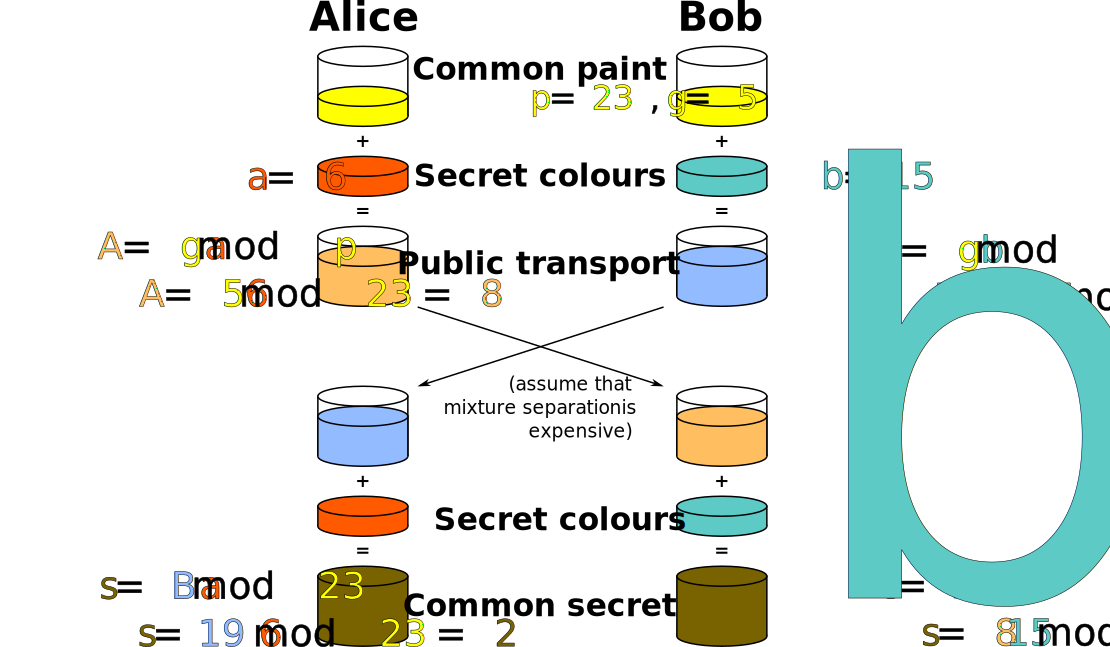
\includegraphics[width=\textwidth]{img/Diffie-Hellman_Key_Exchange_desc}
	\caption{Zobrazowanie działania algorytmu Diffiego-Hellmana (źródło: Wikipedia)}
	\label{fig:dh}
\end{figure}

%---------------------------------------

\subsection{Zestawy kryptograficzne}

W~praktyce, podczas testów, w~czasie których nawiązywano połączenie \gls{ssl/tls} pomiędzy klientem i~serwerem uruchamianym na~systemie z~zainstalowanym \gls{openssl} w~wersji \texttt{1.0.2h}, strony połączenia zawsze negocjowały zestaw algorytmów \texttt{ECDHE-RSA-AES256-GCM-SHA384}, który oznacza użycie najnowszego dostępnej wersji protokołu~\glslink{ssl/tls}{TLS}, tj.~protokołu~TLSv1.2, zapewniającego:
\begin{enumerate}
\item Poufność przez wykorzystanie \gls{aes} pracującym w~trybie GCM z~kluczem o~długości 256~bitów,
\item Ustalenie klucza sesyjnego dla~\gls{aes} przez~wykorzystanie efemerycznej wersji algorytmu \glslink{dh}{Diffiego-Hellmana} w~wersji dla~krzywych eliptycznych~(ECDH),
\item Uwierzytelnienie przez wykorzystanie podpisu cyfrowego z~wykorzystaniem~\gls{rsa},
\item Integralność gwarantowaną przez działanie \gls{aes} w~trybie~GCM. SHA384~w~nazwie wynegocjonowanego zestawu oznacza uczycie funkcji haszującej SHA384 podczas fazy \emph{handshake} i~do rozszerzenia dzielonego sekretu uzyskanego podczas ustalenia klucza~sesyjnego do~klucza symetrycznego dla~\gls{aes}~\cite{stack:openssl-sha-gcm}.
\end{enumerate}

\end{document}
